\subsection{Data Collection}

\subsubsection{Questionnaire}

Our main goal during the data collection process was to obtain GitHub Usernames along with as many answers to questions related to the subject of the recruitment process, assessment of own skills as well as some additional information which could help in the reconstruction of results found in other papers. We have created a Google Form questionnaire and then posted it on two programming-related Facebook Groups.

In both groups, one can find people with a full range of professional experience but based on the activity (posts and comments), one of them is mainly characterized by highly qualified employees (Seniors) while the other seems evenly distributed.

\subsubsection{Parsing GitHub Information}

To collect data from GitHub we used GraphQL Queries \footnote{GraphQL GitHub API: https://docs.github.com/en/graphql}. The query takes only the username on input and on output puts only the information precisely specified within the query itself. GraphQL Query is presented in~\ref{lst:graphql-query} and output format in~\ref{lst:graphql-output-json}.


\begin{lstlisting}[language=R, label={lst:graphql-query}]
{ repositoryOwner(login:"<USER_NAME>") {
    repositories(first: 5, orderBy: {
        field:PUSHED_AT,direction:DESC},
        isFork:false) {
      edges { node {
          name
          diskUsage
          forkCount
          isEmpty
          languages(first : 10){
            edges { size node {
                name
              }
            }
          }
          labels(first : 50){
            totalCount
            nodes{
              name
              description
              updatedAt
            }
          }
          issues (first : 20){
            totalCount
            edges { node {
                body
                author {
                  login
                }
              }
            }
          }
          stargazers {
            totalCount
          }
          description
          defaultBranchRef {
            target{ ... on Commit {
                history(first : 10){
                  totalCount
                  edges { node {
                      ... on Commit {
                        message
                        committedDate
                        author{
                          user{
                            login
    } } } } } } } } } } } }
    ... on User {
      bio
      company
      isHireable
      isViewer
    }
  }
}
\end{lstlisting}

\begin{lstlisting}[language=Python, label={lst:graphql-output-json}]
FUTUREOUTPUT
\end{lstlisting} 

\begin{figure}[htp]
\centering
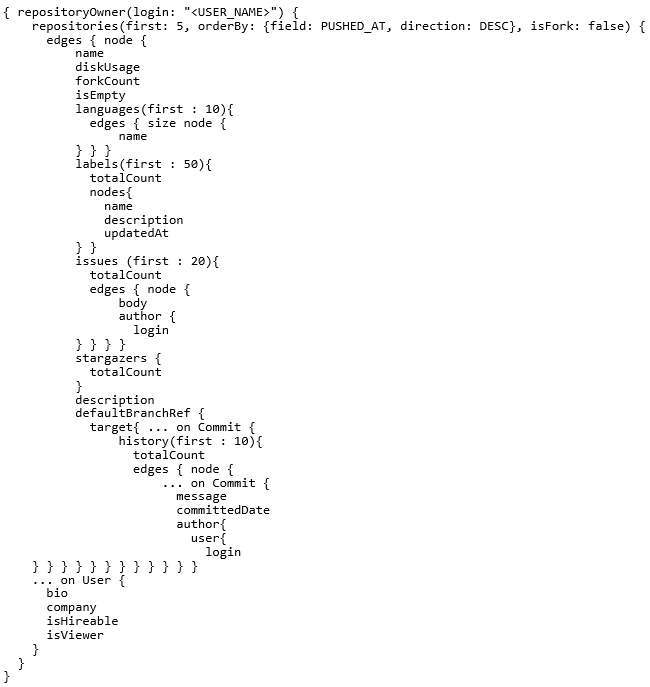
\includegraphics[width=11cm]{query}
\caption{GraphQl Query}
\label{fig:GraphQlQuery}
\end{figure}
